\documentclass[tikz]{standalone}

\usepackage[fontsize=14pt]{fontsize}
\usepackage{tikz}
\usetikzlibrary{matrix,positioning,shapes.arrows,fit}

\begin{document}
	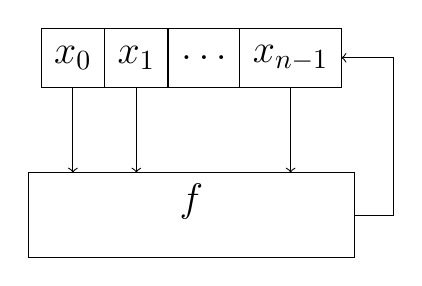
\begin{tikzpicture}[
		every node/.style = {
			draw, rectangle, 
			minimum width=0.75cm,
			minimum height=0.75cm,
			outer sep=0cm, 
			%inner sep=0cm,
			node distance=0cm
			}
		]
		\node (x0) {$x_0$};
		\node [right=of x0.east] (x1) {$x_1$};
		\node [right=of x1.east] (tmp) {$\ldots$};
		\node [right=of tmp.east] (xn1) {$x_{n-1}$};
		
		\node [below=2cm of tmp, fit=(x0.west)(xn1)] (f) {$f$};
		
		\draw[->] (x0.south) -- (x0.south |- f.north);
		\draw[->] (x1.south) -- (x1.south |- f.north);
		\draw[->] (xn1.south) -- (xn1.south |- f.north);
		
		\draw[->] (f.east) -| ++(0.5,0) |- (xn1.east);
		
	\end{tikzpicture}

    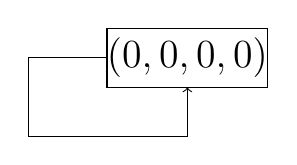
\begin{tikzpicture}[
		every node/.style = {
			draw, rectangle, 
			minimum width=0.75cm,
			minimum height=0.75cm,
			outer sep=0cm, inner sep=0cm,
			node distance=0cm
		}
		]
		\node (s0) {$(0, 0, 0, 0)$};
		\draw[->] (s0.west) -- ++(-1,0) -- ++(0,-1) -| (s0.south);
	\end{tikzpicture}

    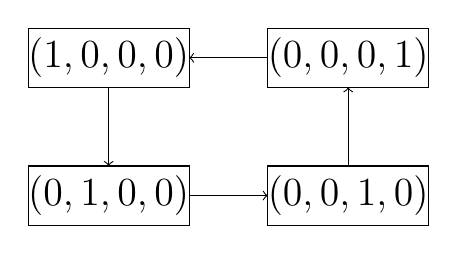
\begin{tikzpicture}[
		every node/.style = {
			draw, rectangle, 
			minimum width=0.75cm,
			minimum height=0.75cm,
			outer sep=0cm, inner sep=0cm,
			node distance=0cm
		}
		]
		\node (s1) {$(0, 0, 0, 1)$};
		\node [left=1cm of s1] (s8) {$(1, 0, 0, 0)$};
		\node [below=1cm of s8] (s4) {$(0, 1, 0, 0)$};
		\node [right=1cm of s4] (s2) {$(0, 0, 1, 0)$};
		\draw[->] (s1.west) -- (s8.east);
		\draw[->] (s8.south) -- (s4.north);
		\draw[->] (s4.east) -- (s2.west);
		\draw[->] (s2.north) -- (s1.south);
	\end{tikzpicture}

    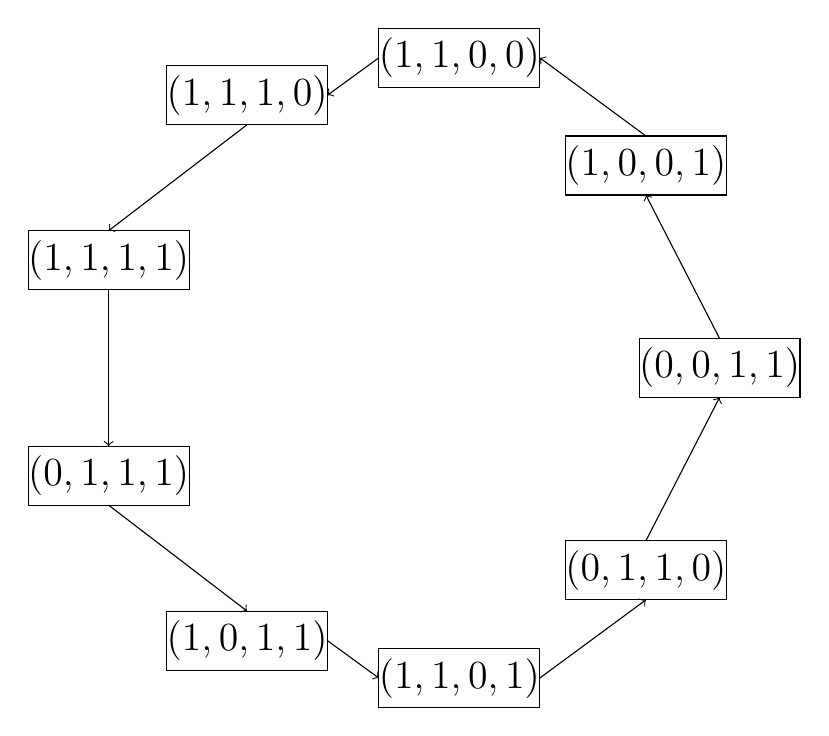
\begin{tikzpicture}[
		every node/.style = {
			draw, rectangle, 
			minimum width=0.75cm,
			minimum height=0.75cm,
			outer sep=0cm, inner sep=0cm,
			%node distance=0cm
		}
		]
		\pgfmathsetmacro\radius{4}
		%\draw (-4,-4) grid (4,4);
		\node (s3) at (\radius*1.0, \radius*0) {$(0, 0, 1, 1)$};
		\node (s9) at ({\radius*cos(1*2*pi/9 r)}, {\radius*sin(1*2*pi/9 r)}) {$(1, 0, 0, 1)$};
		\node (s12) at ({\radius*cos(2*2*pi/9 r)}, {\radius*sin(2*2*pi/9 r)}) {$(1, 1, 0, 0)$};
		\node (s14) at ({\radius*cos(3*2*pi/9 r)}, {\radius*sin(3*2*pi/9 r)}) {$(1, 1, 1, 0)$};
		\node (s15) at ({\radius*cos(4*2*pi/9 r)}, {\radius*sin(4*2*pi/9 r)}) {$(1, 1, 1, 1)$};
		\node (s7) at ({\radius*cos(5*2*pi/9 r)}, {\radius*sin(5*2*pi/9 r)}) {$(0, 1, 1, 1)$};
		\node (s11) at ({\radius*cos(6*2*pi/9 r)}, {\radius*sin(6*2*pi/9 r)}) {$(1, 0, 1, 1)$};
		\node (s13) at ({\radius*cos(7*2*pi/9 r)}, {\radius*sin(7*2*pi/9 r)}) {$(1, 1, 0, 1)$};
		\node (s6) at ({\radius*cos(8*2*pi/9 r)}, {\radius*sin(8*2*pi/9 r)}) {$(0, 1, 1, 0)$};
		
		\draw[->] (s3.north) -- (s9.south);
		\draw[->] (s9.north) -- (s12.east);
		\draw[->] (s12.west) -- (s14.east);
		\draw[->] (s14.south) -- (s15.north);
		\draw[->] (s15.south) -- (s7.north);
		\draw[->] (s7.south) -- (s11.north);
		\draw[->] (s11.east) -- (s13.west);
		\draw[->] (s13.east) -- (s6.south);
		\draw[->] (s6.north) -- (s3.south);
	\end{tikzpicture}

    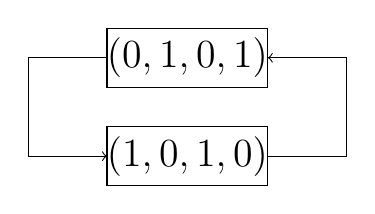
\begin{tikzpicture}[
		every node/.style = {
			draw, rectangle, 
			minimum width=0.75cm,
			minimum height=0.75cm,
			outer sep=0cm, inner sep=0cm,
			node distance=0cm
		}
		]
		\node (s5) {$(0, 1, 0, 1)$};
		\node [below=0.5cm of s5](s10) {$(1, 0, 1, 0)$};
		\draw[->] (s5.west) -- ++(-1,0) |- (s10.west);
		\draw[->] (s10.east) -- ++(1, 0) |- (s5.east);
	\end{tikzpicture}
\end{document}